\documentclass[10pt,twocolumn,letterpaper]{article}
\usepackage{cite} 
\usepackage{iccv}
\usepackage{times}
\usepackage{epsfig}
\usepackage{graphicx}
\usepackage{amsmath}
\usepackage{amssymb}



% Include other packages here, before hyperref.

% If you comment hyperref and then uncomment it, you should delete
% egpaper.aux before re-running latex.  (Or just hit 'q' on the first latex
% run, let it finish, and you should be clear).
\usepackage[pagebackref=true,breaklinks=true,letterpaper=true,colorlinks,bookmarks=false]{hyperref}

% \iccvfinalcopy % *** Uncomment this line for the final submission

\def\iccvPaperID{****} % *** Enter the ICCV Paper ID here
\def\httilde{\mbox{\tt\raisebox{-.5ex}{\symbol{126}}}}

% Pages are numbered in submission mode, and unnumbered in camera-ready
\ificcvfinal\pagestyle{empty}\fi

\begin{document}

%%%%%%%%% TITLE
\title{Extreme Memory Cost Reduction of CNN Training by Reversible Neural Network }

\author{First Author\\
Institution1\\
Institution1 address\\
{\tt\small firstauthor@i1.org}
% For a paper whose authors are all at the same institution,
% omit the following lines up until the closing ``}''.
% Additional authors and addresses can be added with ``\and'',
% just like the second author.
% To save space, use either the email address or home page, not both
\and
Second Author\\
Institution2\\
First line of institution2 address\\
{\tt\small secondauthor@i2.org}
}

\maketitle
% Remove page # from the first page of camera-ready.
\ificcvfinal\thispagestyle{empty}\fi

%%%%%%%%% ABSTRACT
\begin{abstract}
   Recently, Convolutional Neural Networks (CNN) have demonstrated state-of-the-art results on various computer vision problems. However, training CNNs require specialized GPU with large memory. Given the ubiquity of CNN in computer vision, optimizing the memory consumption of CNN training would have wide spread practical benefits. GPU memory is a major bottleneck of the CNN training procedure, limiting the size of both inputs and model architectures. Recently, reversible neural networks have been proposed to solve memory bottleneck problem by recompute input activations by inverse operation. In this paper, we summary previous research and push those idea to extreme and design a reversible neural network with minimal GPU memory consumption while training neural network. The result demonstrated that we can train CIFAR10 dataset on Nvidia GTX750 GPU only with 1GB memory and achieve 93\% accuracy within 67 minutes.
   
   
\end{abstract}

%%%%%%%%% BODY TEXT

\section{Introduction}
  Since Krizhevsky et al., won the 2012 ILSVRC, CNN have been successfully applied to many different real-world applications. However, training state-of-the-art CNN has required special hardware with large memory capacity as typical desktop memory is too small for backpropagation training. Therefore, the barrier to entry into deep learning research costs either purchasing specialized hardware or renting real-time instances from cloud service providers. However, training in cloud servers could not be a preferred choice while involve private data. On-device training would allow fine-tuning neural network models on local data without sending sensitive data over the network.

  Reducing the memory consumption is necessary that would train neural networks efficiently in standard GPU without this barrier of bottleneck. Meanwhile, a number or recent work have demonstrated the benefits of large batch training \cite{largebatch}, training in Imagenet increase batch sizes up to tens of thousands of samples, training speed would linear speed-ups as well that further increasing these memory requirements. Hence optimizing the memory usage of CNN training would enable both research on optimization and training on low-end GPU devices.

  There is an inherent trade-off between memory consumption and computation time: gradient checkpointing methods \cite{chen2016training} only store a fraction of the hidden activations and reconstructing the missing activations from the stored ones during the backward pass.
  
   Reversible Network (RevNet) \cite{gomez2017reversible} constrain the architecture of Residual Networks to invertible transformations so that each layer’s input activations are reconstructed from their output during the backward pass.
  However, two factors create memory bottlenecks in training RevNet, the gradient of activations have to wait for the full reversible block recomputation that is local bottleneck. RevNet features non-volume preserving max-pooling layers, for which the inverse cannot be computed, their input must stored in memory that we call global bottleneck. 
  
  The iRevNet \cite{jacobsen2018revnet} model builds on the RevNet architecture: they replace the irreversible max-pooling with an invertible operation. One downside of their method is that the proposed invertible pooling scheme drastically increases the number of channels in upper layers with the size of the convolution kernel weights grows quadratically, the memory cost associated with storing the model weights becomes a major memory bottleneck. 
  
 In this paper,we use the ResNet-18 as a research starting point to analyse its training memory requirement. Then We introduce a layer-wise invertible architecture and characterize the accumulate numerical errors across their layers, which leads to numerical instabilities impacting model accuracy. We proposed a hybrid architecture consist of layer-wise and residual-block that allow us to efficiently train CNN model by circumvent those bottleneck. The result show that training our hybrid model could achieve 93.3\% accuracy on CIFAR10 dataset in 67 minutes on low-end Nvidia GTX750 GPU only with 1GB memory.  
    

%\section{Related Work}
%Several approaches have been proposed to reduce memory usage and computation consumption. MobileNet\cite{howard2017mobilenets} is a light neural network using depth-wise separable convolution to reduce computation complexity to perform inference on low performance device. Quantized Neural Network (QNN)\cite{hubara2017quantized} is designed to reduce memory by performing low-precision arithmetic operations. Network pruning\cite{molchanov2016pruning} is a set of techniques developed to decrease the model weight size and computational complexity. Network pruning works by removing the network weights that contribute the least to the model output.
%	
%Most related to our work, gradient checkpointing is an efficient trick for reducing CNN memory usage: it only stores a few of the hidden layers input activations during the forward pass and reconstruct the lost activations during the backward pass.
%	
%RevNet recompute the hidden activation of lower layers from those of higher layers. Hence, activations need not to be stored during the forward pass as they can be recomputed during the backward pass. However, two factors create memory bottlenecks in training RevNet, which we refer to as the local and global bottlenecks. The gradient of activations have to wait for the full reversible block recomputation that is local bottleneck. RevNet features non-volume preserving max-pooling layers, for which the inverse cannot be computed, their input must stored in memory that we call global bottleneck. 
%
%The iRevNet \cite{jacobsen2018revnet} model builds on the RevNet architecture: they replace the irreversible max-pooling with an invertible operation. As such, the iRevNet architecture is fully invertible, which alleviates the global memory bottleneck of the RevNet architecture. From a resource optimization point of view, one downside of their method is that the proposed invertible pooling scheme drastically increases the number of channels in upper layers with the size of the convolution kernel weights grows quadratically, the memory cost associated with storing the model weights becomes a major memory bottleneck. We address this issue in our proposed architecture.



\section{Memory footprint}
We denote the memory footprint of training a neural network as a value $\mathcal{M}$ in bytes. The memory footprint represents the peak memory consumption during an iteration of training forward and backward pass. Total memory footprint  $\mathcal{M}$ consist of:  model weights, hidden activations and gradients.
    
The vanilla ResNet-18 do not use reversible computations so that the input activations need to be accumulated in memory during the forward pass for the computation of the weight gradients during in backward pass. Hence the peak memory footprint of training a vanilla ResNet happens at the beginning of the backward pass.

For example, train a typical batch of 32, RGB image of $240 \times 240$ requires 12.5 MB  store the model weights and 3.8 GB of hidden layers activation and gradient for a total of  $\mathcal{M}$ = 3.81 GB.The memory cost of the hidden activations is thus the main memory bottleneck of CNN training. 
 
Reversible blocks have analytical inverses that allow recomputation of both their input and hidden activations. And the peak memory consumption of RevNet, happens in the backward pass through the first reversible block. Following our previous example, a RevNet closely mimicking the ResNet-18 requires $\mathcal{M}$ = 1.19 GB and 12.7 MB weights. However, RevNet trade memory for computation time, as noted in original paper, this computation cost equivalent performing one additional forward pass.

The iRevNet is fully invertible by use irreversible max-pooling to alleviates the global bottleneck. But, it requires 171 MB weights and $\mathcal{M}$ = 1.35 GB. At this point, the memory cost of weights becomes an additional memory bottleneck. Furthermore, the iRevNet does not address the local memory bottleneck of reversible blocks. 

\section{Methods} 
RevNet and iRevNet which we have seen in the previous section, their design still create a local memory as all hidden activations need to be computed before the gradients are backpropagated. In order to circumvent this local memory bottleneck, we introduce layer-wise invertible operations. However, these invertible operations introduce numerical error. Hence, we propose a hybrid model combining layer-wise and block-wise reversible operation to resolve the local memory bottleneck at the cost of a small additional computation cost.


\subsection{Layer-wise invertibility}
\subsubsection{Invertible batch normalization}
%batch normalization%
As batch normalization is not a bijective operation, it does admit an analytical inverse. However, the output recovered by upstream invertible layers is a noisy of the true output due to numerical errors introduced by upstream layers.
  
We characterize the factor $\alpha $ of reduction of signal to noise ratio (SNR) through the inverse reconstruction. 
Let us consider a toy layer with only two channels and parameters $\beta=[0,0]$ and $\gamma = [1, \rho]$ of first and second order moment parameters $\beta$ and $\gamma$. 
For simplicity, let us consider an input signal $x$ independently and identically distributed across both channels 
with zero mean and standard deviation 1 so that, in the forward pass, we have:

\begin{equation}
\alpha = \frac{4}{(1+\frac{1}{\rho^2}) \times (1 + \rho^2)}
\end{equation} 

\begin{figure}[h]
\begin{center}
\includegraphics[height=0.5\linewidth]{Figure5.eps}
\end{center}
   \caption{Illustration of the numerical errors arising from batch normalization layers.}
\end{figure}
Figure 1 shows the expected evolution of $\alpha$ through our toy layer for different values of the factor $\rho$.
To validate our formula, we empirically evaluate $\alpha$ for normal Gaussian inputs $x$ and output noise $\epsilon^y$ and find it to closely match the theoretical results given by equation 1.
\subsubsection{Invertible activation function}
%activation function%
  A good invertible activation function must be bijective (to guarantee the existence of an inverse function). For these properties, we focus our attention on Leaky ReLUs.
  The analysis of the numerical errors yielded by the invertible Leaky ReLU follows a similar reasoning as the toy batch normalization example with an additional subtlety: We can think of the leaky ReLU as artificially splitting the input x across two different channels, 
one channel leaving the output unchanged and one channel that divides the input by a factor $n$ during the forward pass and multiplies its output by a factor $n$ during the backward pass.
The signal to noise ration reduction factor $\alpha$ can be expressed as:

\begin{equation}
\alpha = \frac{4}{(1+\frac{1}{n^2}) \times (1 + n^2)}
\end{equation}

Hence numerical errors can be controlled by setting the value of the negative slope $n$.
Figure 2 shows the evolution of the SNR degradation $\alpha$ for different negative slopes $n$; 

\begin{figure}[h]
\begin{center}
\includegraphics[height=0.5\linewidth]{Figure6.eps}
\end{center}
   \caption{Illustration of the numerical errors arising from invertible activation layers.}
\end{figure}

\subsubsection{Pooling}
%pooling
In iRevNet, the authors propose an invertible pooling operation that operates by stacking the neighboring elements of the pooling regions along the channel dimension. 

We propose a new pooling layer that stacks the elements of neighboring pooling regions along the batch size instead of the channel size to circumvent quadratic increase in weight memory. 
We refer to both kind of pooling as channel pooling $\mathcal{P}_c$ and batch pooling $\mathcal{P}_b$ respectively. The reshaping operation performed by both pooling layers can be formalized as follows:

\begin{subequations}
\begin{align}
	\mathcal{P}_c :&  \mathbb{R}^{bs \times c \times h \times w}  \rightarrow \mathbb{R}^{bs \times 4c \times \frac{h}{2} \times \frac{w}{2}}\\
	\mathcal{P}_b :&  \mathbb{R}^{bs \times c \times h \times w}  \rightarrow \mathbb{R}^{4bs \times c \times \frac{h}{2} \times \frac{w}{2}}
\end{align}
\end{subequations}

The $bs$ refers to the batch size, $c$ to the number of channels and $h \times w$ to the resolution.
\subsubsection{Invertible convolutions}
Deconvolution is a way of invertible convolution. However, deconvolution is computationally expensive. We choose to implement invertible convolutions using the channel partitioning scheme as the reversible block design. Hence in our architecture, invertible convolutions, can be seen as minimal reversible blocks in which both modules consist of a single convolution. Gomez found the numerical errors introduced by reversible blocks to have no impact on the model accuracy.
%\begin{figure}[h]
%\begin{center}
%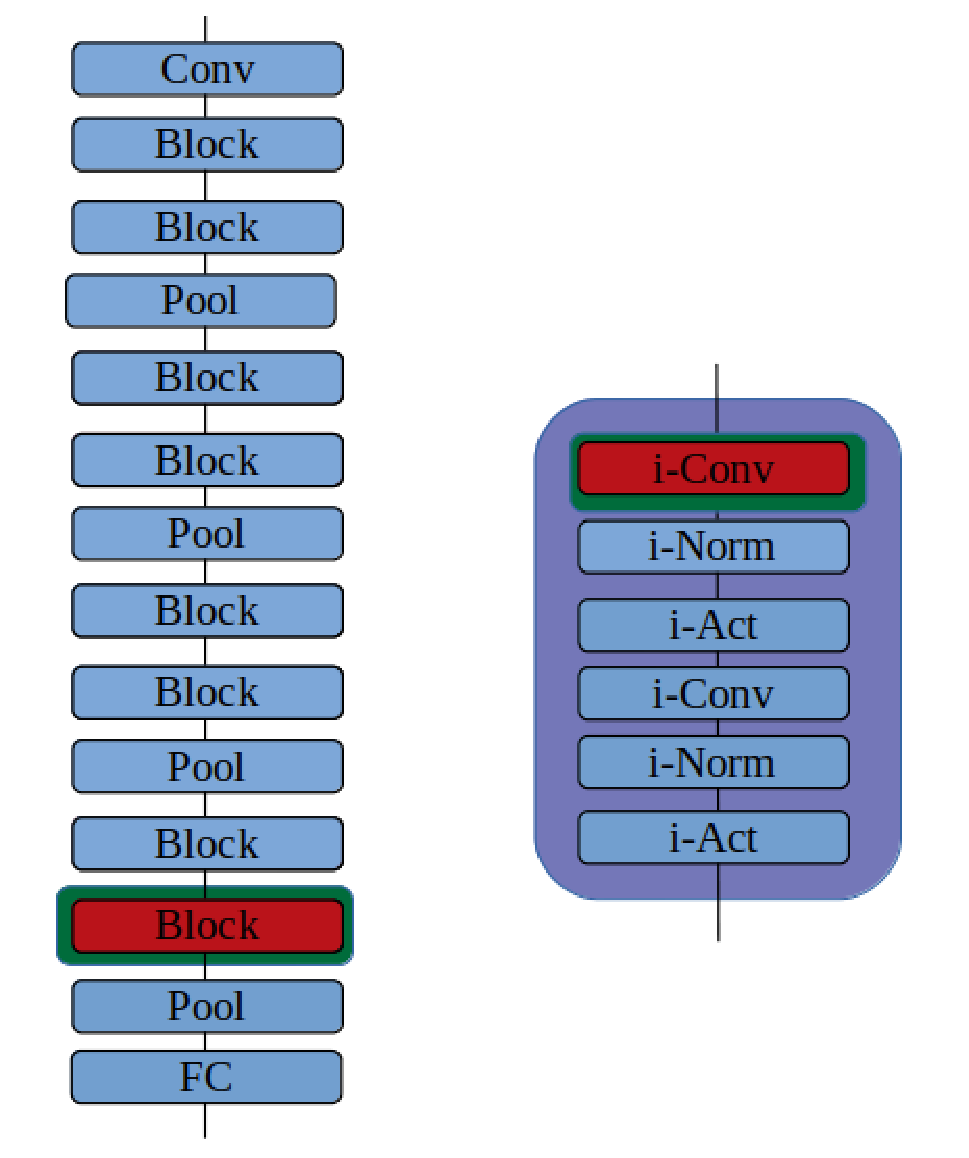
\includegraphics[height=0.5\linewidth]{Figure2.eps}
%\end{center}
%   \caption{Illustration of a layer-wise invertible architecture and
%its memory consumption.}
%\end{figure}

\begin{table*}[t]
\begin{center}
\caption{Summary of architectures with different levels of reversibility}
\begin{tabular}{ c c c c c c}	
Model     & Accuracy & \#Params & Channels & Pooling & $\mathcal{M} $ \\
\hline
Resnet    & $94.7\%$   & $3.1M$   &  $32 - 64 - 128  - 256$       & Max Pooling     & $1.01G$  \\			
RevNet    & $94.5\%$   & $3.1M$   &  $40 - 80 - 256  - 320$       & Max Pooling     & $348M$   \\
i-RevNet  & $93.8\%$   & $42.8M$  &  $32 - 128 - 512 - 2048$      & $\mathcal{P}_c - \mathcal{P}_c - \mathcal{P}_c$  & $500M$   \\
Ours      & $93.3\%$   & $3.7M$   &  $32 - 128 - 512 - 512$       & $[\mathcal{P}_c, \mathcal{P}_c, \mathcal{P}_b]$  & $200M$   \\
\hline
\end{tabular}
\end{center}
\end{table*}

\subsubsection{Layer-wise invertible architecture}
Putting together the above building blocks. The peak memory usage for training iteration of this architecture requires $\mathcal{M}$ = 590 MB including 29.6 MB gradients. Similar to RevNet, the recomputation of activations during the backward pass comes with an additional computational cost similar to a forward pass.

In Figure 3, we compare the evolution of the accuracy in both settings for different depth and negative slopes.
For small depths (or high negative slopes), in which the numerical errors are minimum, both models yield similar accuracy.

\begin{figure}[h]
\begin{center}
\includegraphics[width=1\linewidth]{Figure7.eps}
\end{center}
   \caption{Impact of the numerical errors on the accuracy of layer-wise invertible models.}
\end{figure}




\subsection{Hybrid architecture}
\begin{figure}[h]
\begin{center}
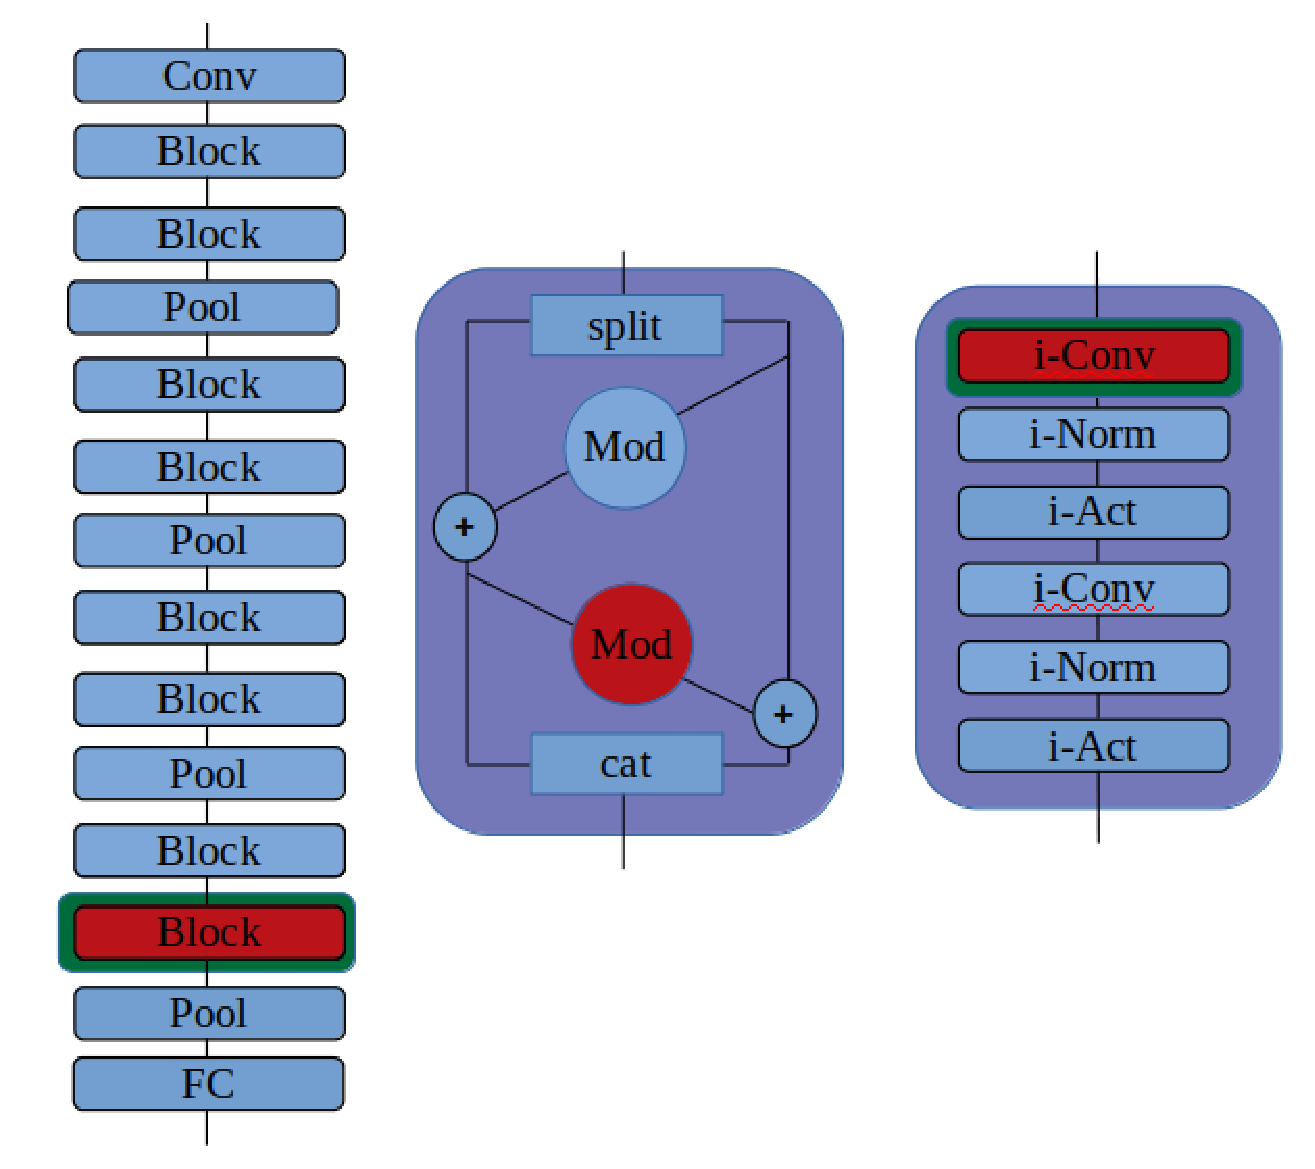
\includegraphics[height=0.5\linewidth]{Figure3.eps}
\end{center}
   \caption{Illustration of a hybrid architecture and its peak
memory consumption.}
\end{figure}
Through long chains of layer-wise invertible operations will accumulate numerical errors and show that numerical errors negatively impact model accuracy. To prevent these numerical instabilities, we introduce a hybrid architecture.Figure 4 illustrate our hybrid architecture, combining reversible residual blocks with layer-wise invertible function. Conceptually, the role of the layer-wise invertible layers is to efficiently recompute the hidden activations within the reversible residual blocks at the same time as the gradient propagates to circumvent the local memory bottleneck of the reversible module. 

Figure 5 illustrate the backward pass though the hybrid reversible block. The backward pass is made of two phases: 
First the input activations are recomputed from the output using the Reversible block analytical inverse (middle).
During this step, hidden activations are not kept in live memory so as to avoid the local memory bottleneck of the reversible block.
Once the input activation recomputed, the gradients are propagated backward through both modules of the reversible blocks (right).
During this second phase, hidden activations are recomputed backward through each module using the layer-wise inverse operations, yielding minimal memory footprint.




\begin{figure}[h]
\begin{center}
%\fbox{\rule{0pt}{2in} \rule{0.9\linewidth}{0pt}}
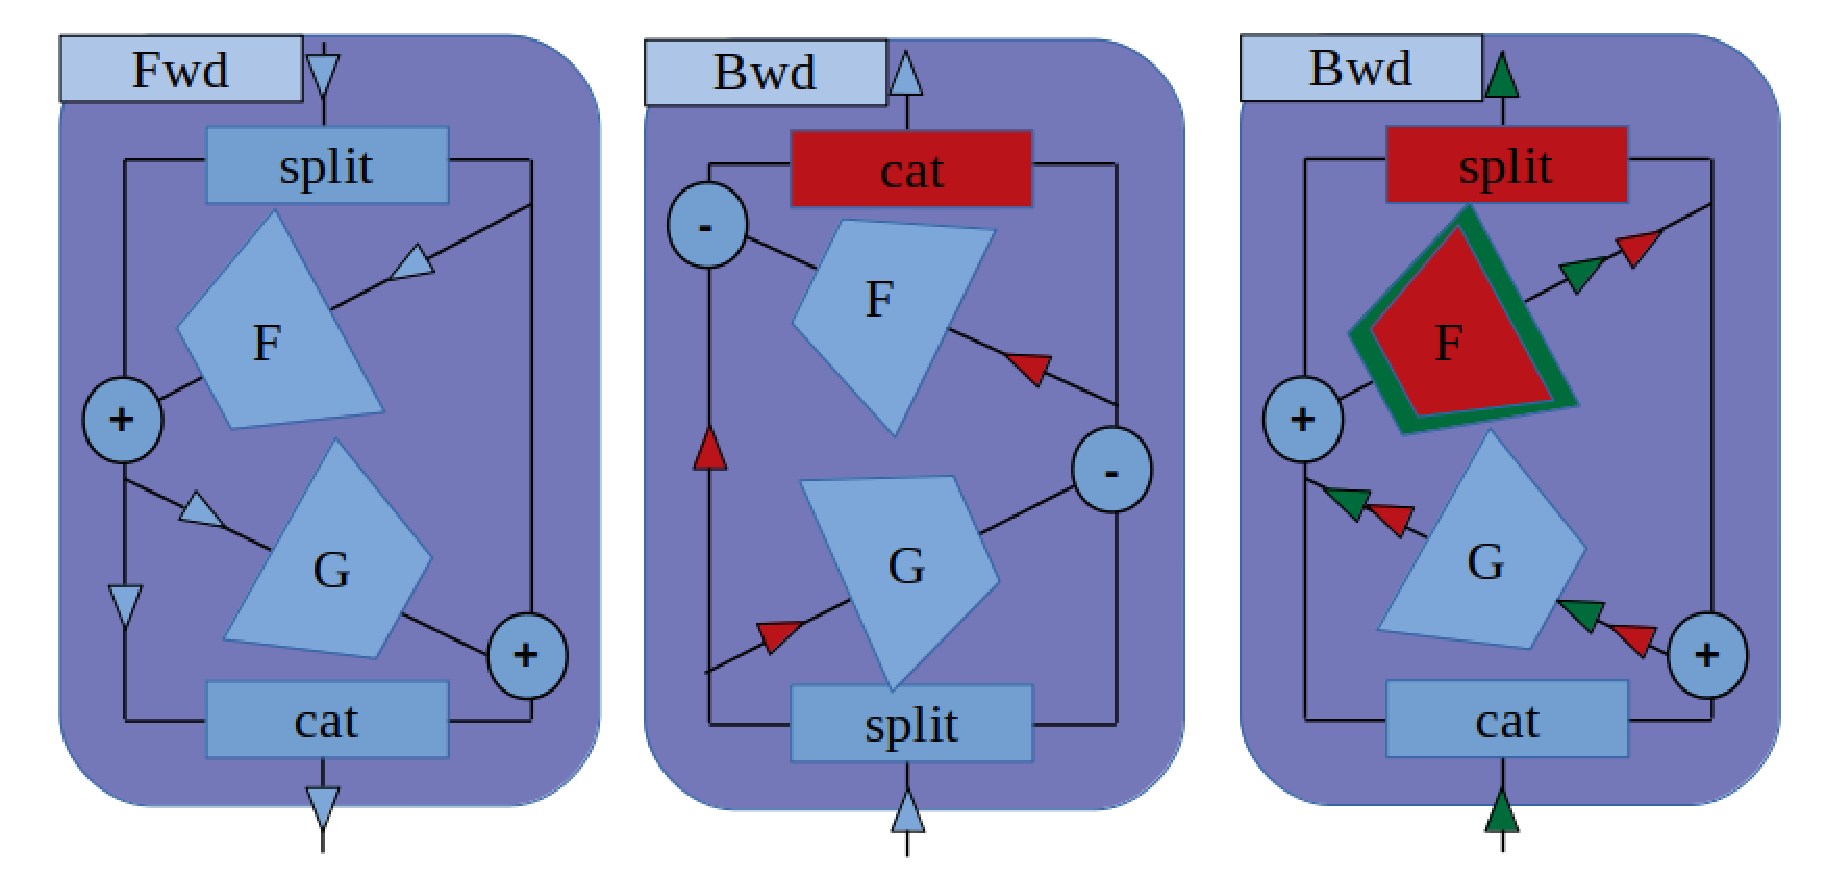
\includegraphics[width=0.5\linewidth]{Figure4.eps}
\end{center}
   \caption{Illustration of the backpropagation process through a
reversible block of our proposed hybrid architecture.}
%\label{fig:long}
%\label{fig:onecol}
\end{figure}
As each layer within these modules is invertible, the hidden activations are computed using the layer-wise inverse along the gradient. The layer-wise inversion allows us to alleviate the local bottleneck of the reversible block by computing the hidden activation values together with the backward flow of the gradients. The peak memory consumption of our proposed architecture, training an iteration over batch of 32 images of resolution 240$\times$240 would require $\mathcal{M}$ = 648MB including 14.8 MB weights.

It should be noted, instead of one additional forward pass, as in the RevNet and layer-wise architectures, our hybrid architecture comes with a computational cost equivalent to performing two additional forward passes during the backward pass. 

\section{Results} 
We use the CIFAR10 dataset as a benchmark for our experiments. The CIFAR10 dataset is complex enough to require efficient architectures to reach high accuracy, yet small enough to enable us to rapidly iterate over different architectural designs. 

We summarize the benefits and drawbacks of our proposed architecture in comparison to different baseline architectures. Table 1 summarizes our main results. In this table, we compare architectures with different patterns of reversibility. To allow for a fair comparison, we have tweaked each architecture to keep the number of parameters as close as possible.

All models were trained for 50 epochs of stochastic gradient descent with cyclical learning rate and momentum with minimal image augmentation.

Compared to the original ResNet architecture, our model drastically cuts the memory cost of training. These drastic memory cuts come at the cost of a small degradation in accuracy.

Furthermore, our hybrid architecture requires two equivalent additional forward computation within each backward pass. In Table 2, we compare the time of training our hybrid architecture to 93.3\% accuracy on Nvidia GTX1080Ti and low-end Nvidia GTX750 GPU which only has 1 GB memory and roughly 400 MB of available memory after the initialization of various frameworks. It is impractical train a vanilla ResNet with large batch size, while our architecture allows for efficient training.
\begin{table}[t]
\centering
\caption{Training statistics on different hardware}
\begin{tabular}{ c c c c}	
 GPU & Accuracy  & Time \\
\hline			
GTX750     & $93.3\%$  & $67 min$    \\
GTX 1080Ti & $93.3\%$  & $37min$  \\
\hline
\end{tabular}
\end{table}

\section{Conclusion} 
Convolutional Neural Networks have become the backbone of computer vision systems. Despite their great success, one major drawback of these models is their intense resource consumption: Training CNNs needs highly optimized implementations leveraging all possible hardware resources. In this paper, we have presented an architecture able to yield high accuracy classifications within very tight memory constraints and train a hybrid CNN model to 93.3\% accuracy on a low-end GPU only 1 GB memory.


{\small
\bibliographystyle{ieeetr}
\bibliography{iccv_paper_review}
}
\end{document}
